\chapter*{Dasar Teori}
\addcontentsline{toc}{chapter}{Dasar Teori}

\section{Latar Belakang dan Relevansi}
Di sistem pendidikan kita sekarang, bantuan untuk siswa yang kesulitan seringkali datang terlambat. Biasanya, sekolah baru akan bertindak---misalnya dengan mengadakan kelas remedial---setelah nilai ujian akhir keluar dan hasilnya kurang memuaskan. Tentu saja, pendekatan seperti ini punya kelemahan besar: bantuan diberikan saat semuanya sudah terjadi, di mana siswa mungkin sudah kehilangan motivasi.
Di sinilah \textit{machine learning} bisa mengubah keadaan. Dengan menganalisis data-data siswa yang sudah ada---mulai dari data pribadi, pergaulan, dan terutama nilai-nilai sebelumnya---kita bisa membuat sebuah model prediksi. Model ini bisa berfungsi seperti ``sistem peringatan dini'' yang bisa menandai siswa mana yang kemungkinan besar akan gagal, jauh sebelum ujian akhir. Dengan kemampuan ini, para guru bisa memberikan bantuan yang lebih personal dan tepat waktu, sehingga peluang siswa untuk berhasil jadi lebih besar.

\section{Tujuan dan Ruang Lingkup Proyek}
Berdasarkan masalah di atas, tujuan utama dari proyek ini adalah:
\begin{enumerate}
    \item Membuat dan melatih beberapa model \textit{machine learning} untuk memprediksi nilai akhir matematika siswa (\texttt{G3}).
    \item Membandingkan model-model tersebut untuk menemukan mana yang paling akurat dan bisa diandalkan.
    \item Menganalisis fitur atau faktor apa saja yang paling berpengaruh menurut model terbaik.
\end{enumerate}

Untuk mencapai tujuan itu, proyek ini punya batasan (ruang lingkup) sebagai berikut:
\begin{itemize}
    \item \textbf{Dataset:} Kami menggunakan dataset publik ``Student Performance'' dari UCI, yang berisi data dari 395 siswa di Portugal.
    \item \textbf{Metodologi:} Kami mengikuti alur kerja standar, mulai dari membuat fitur baru (\textit{feature engineering}), memproses data (\textit{preprocessing}), hingga melatih model.
    \item \textbf{Model yang Diuji:} Kami membandingkan beberapa jenis model: \textbf{Regresi Linear} (sebagai baseline), \textbf{Random Forest} dan \textbf{XGBoost} (sebagai model ensemble canggih), serta \textbf{Multi-Layer Perceptron (MLP)} (sebagai perwakilan deep learning).
    \item \textbf{Metrik Evaluasi:} Performa model diukur menggunakan \textbf{R-squared (R²)} dan \textbf{Root Mean Squared Error (RMSE)}.
\end{itemize}

Pendekatan untuk membandingkan berbagai model seperti ini sejalan dengan banyak penelitian di bidang \textit{Educational Data Mining}. Sebagai contoh, sebuah studi oleh Al-Barrak dan Al-Razgan (2016) juga membandingkan beberapa algoritma, termasuk \textit{Decision Trees} (yang menjadi dasar dari Random Forest dan XGBoost), untuk memprediksi IPK mahasiswa. Studi mereka juga menemukan bahwa nilai-nilai sebelumnya adalah faktor prediksi terkuat, sebuah temuan yang menjadi fondasi utama dalam analisis kami.

\section*{Referensi}
Al-Barrak, M. A., \& Al-Razgan, M. (2016). Predicting Students Final GPA Using Decision Trees: A Case Study. \textit{International Journal of Information and Education Technology, 6}(7), 528-533. doi:10.7763/IJIET.2016.V6.745.

\vspace{0.2cm}
Cortez, P. (2008). Student Performance [Dataset]. UCI Machine Learning Repository. https://doi.org/10.24432/C5TG7T.

\vspace{0.5cm}
Dengan landasan teori ini, langkah selanjutnya adalah memahami secara mendalam dataset yang akan digunakan dalam proyek ini.

\chapter*{DataSet}
\addcontentsline{toc}{chapter}{DataSet}

\section{Deskripsi Dataset}
Dataset yang kami pilih untuk proyek ini, yaitu ``Student Performance Data Set'', lebih dari sekadar nilai-nilai tak bermakna. Ini adalah potret lengkap kehidupan para siswa. Keistimewaannya adalah data yang sangat beragam, mencakup semuanya mulai dari nilai-nilai akademik, data diri (seperti usia dan alamat), latar belakang keluarga (seperti pendidikan orang tua), hingga gaya hidup mereka (seperti waktu belajar, absensi, dan seberapa sering mereka main). Karena datanya begitu kaya dan bervariasi, ini menjadi dasar yang sempurna untuk membuat model prediksi yang bagus dan menggali faktor apa saja yang sebenarnya mengukur kesuksesan akademis seorang siswa.

\subsection{Sumber Data}
\begin{itemize}
    \item \textbf{Judul:} Student Performance Data Set
    \item \textbf{Author:} P. Cortez and A. Silva
    \item \textbf{Tanggal Terbit:} 2008
    \item \textbf{Sumber:} UCI Machine Learning Repository
    \item \textbf{Relevansi:} Dataset ini sangat relevan karena secara spesifik mencatat berbagai atribut demografis, sosial, dan akademik siswa yang dapat digunakan untuk tujuan prediksi kinerja, sejalan dengan tujuan proyek ini.
\end{itemize}

\subsection{Ukuran dan Kualitas Dataset}
\begin{itemize}
    \item \textbf{Jumlah Data:} Dataset ini terdiri dari \textbf{395 entri} (siswa).
    \item \textbf{Jumlah Fitur:} Terdapat total \textbf{33 fitur} (atribut) awal untuk setiap siswa.
    \item \textbf{Data Kosong:} Analisis awal menunjukkan bahwa dataset ini memiliki kualitas yang sangat baik, dengan \textbf{tidak ada nilai kosong} (\textit{missing values}) sama sekali, sehingga tidak memerlukan langkah mengeluarkan data.
\end{itemize}

\subsection{Fitur-fitur Relevan}
Berikut adalah deskripsi dari fitur-fitur utama yang terdapat dalam dataset:
\begin{longtable}{|p{0.15\linewidth}|p{0.15\linewidth}|p{0.6\linewidth}|}
    \hline
    \textbf{Nama Variabel} & \textbf{Tipe Data} & \textbf{Deskripsi} \\
    \hline
    \endhead
    school & Kategorikal & Sekolah siswa (`GP' atau `MS') \\
    sex & Biner & Jenis kelamin siswa (`F' atau `M') \\
    age & Integer & Usia siswa (15 hingga 22) \\
    address & Kategorikal & Tipe alamat rumah (`U' - urban atau `R' - rural) \\
    famsize & Kategorikal & Ukuran keluarga (`LE3' - <=3 atau `GT3' - >3) \\
    Pstatus & Kategorikal & Status kohabitasi orang tua (`T' - bersama atau `A' - berpisah) \\
    Medu & Integer & Pendidikan Ibu (0 - tidak ada, 4 - pendidikan tinggi) \\
    Fedu & Integer & Pendidikan Ayah (0 - tidak ada, 4 - pendidikan tinggi) \\
    Mjob & Kategorikal & Pekerjaan Ibu (`teacher', `health', `services', dll.) \\
    Fjob & Kategorikal & Pekerjaan Ayah (`teacher', `health', `services', dll.) \\
    studytime & Integer & Waktu belajar mingguan (1 - <2 jam, 4 - >10 jam) \\
    failures & Integer & Jumlah kegagalan kelas sebelumnya (0-4) \\
    schoolsup & Biner & Dukungan pendidikan ekstra dari sekolah (yes/no) \\
    famsup & Biner & Dukungan pendidikan dari keluarga (yes/no) \\
    activities & Biner & Mengikuti kegiatan ekstrakurikuler (yes/no) \\
    higher & Biner & Ingin melanjutkan ke pendidikan tinggi (yes/no) \\
    internet & Biner & Akses internet di rumah (yes/no) \\
    romantic & Biner & Dalam hubungan romantis (yes/no) \\
    famrel & Integer & Kualitas hubungan keluarga (1 - sangat buruk, 5 - sangat baik) \\
    goout & Integer & Frekuensi pergi keluar bersama teman (1 - sangat jarang, 5 - sangat sering) \\
    health & Integer & Status kesehatan saat ini (1 - sangat buruk, 5 - sangat baik) \\
    absences & Integer & Jumlah absensi sekolah (0 hingga 93) \\
    G1 & Target & Nilai periode pertama (0 hingga 20) \\
    G2 & Target & Nilai periode kedua (0 hingga 20) \\
    G3 & Target & Nilai akhir (0 hingga 20) --- **Output Target Utama** \\
    \hline
    \caption{Deskripsi Fitur dalam Dataset}
\end{longtable}

\section{Langkah Preprocessing dan Transformasi Data}
Data mentah diolah melalui beberapa tahapan kunci untuk memaksimalkan potensinya dalam pemodelan.

\subsection{Eksplorasi Data (EDA)}
Langkah awal ini krusial untuk memahami data. Dengan membuat visualisasi seperti histogram dan heatmap, kami dapat mengidentifikasi pola, distribusi data, serta korelasi antar fitur. Wawasan dari EDA, seperti korelasi kuat antara G1/G2 dengan G3, menjadi dasar untuk pemilihan fitur di tahap selanjutnya.
\begin{figure}[h!]
    \centering
    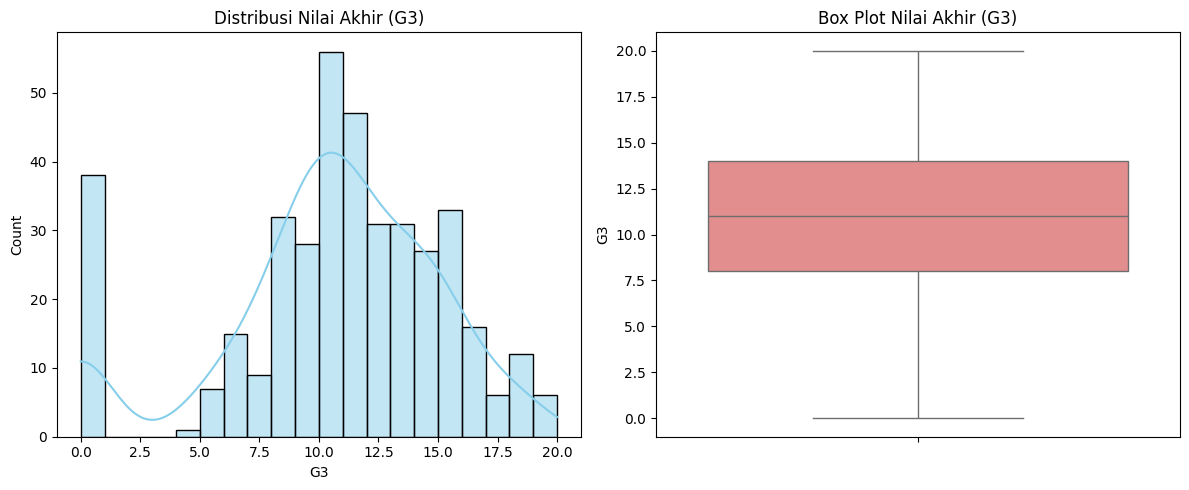
\includegraphics[width=0.8\textwidth]{images/G3Dist.png}
    \caption{Distribusi value G3}
\end{figure}
\begin{figure}[h!]
    \centering
    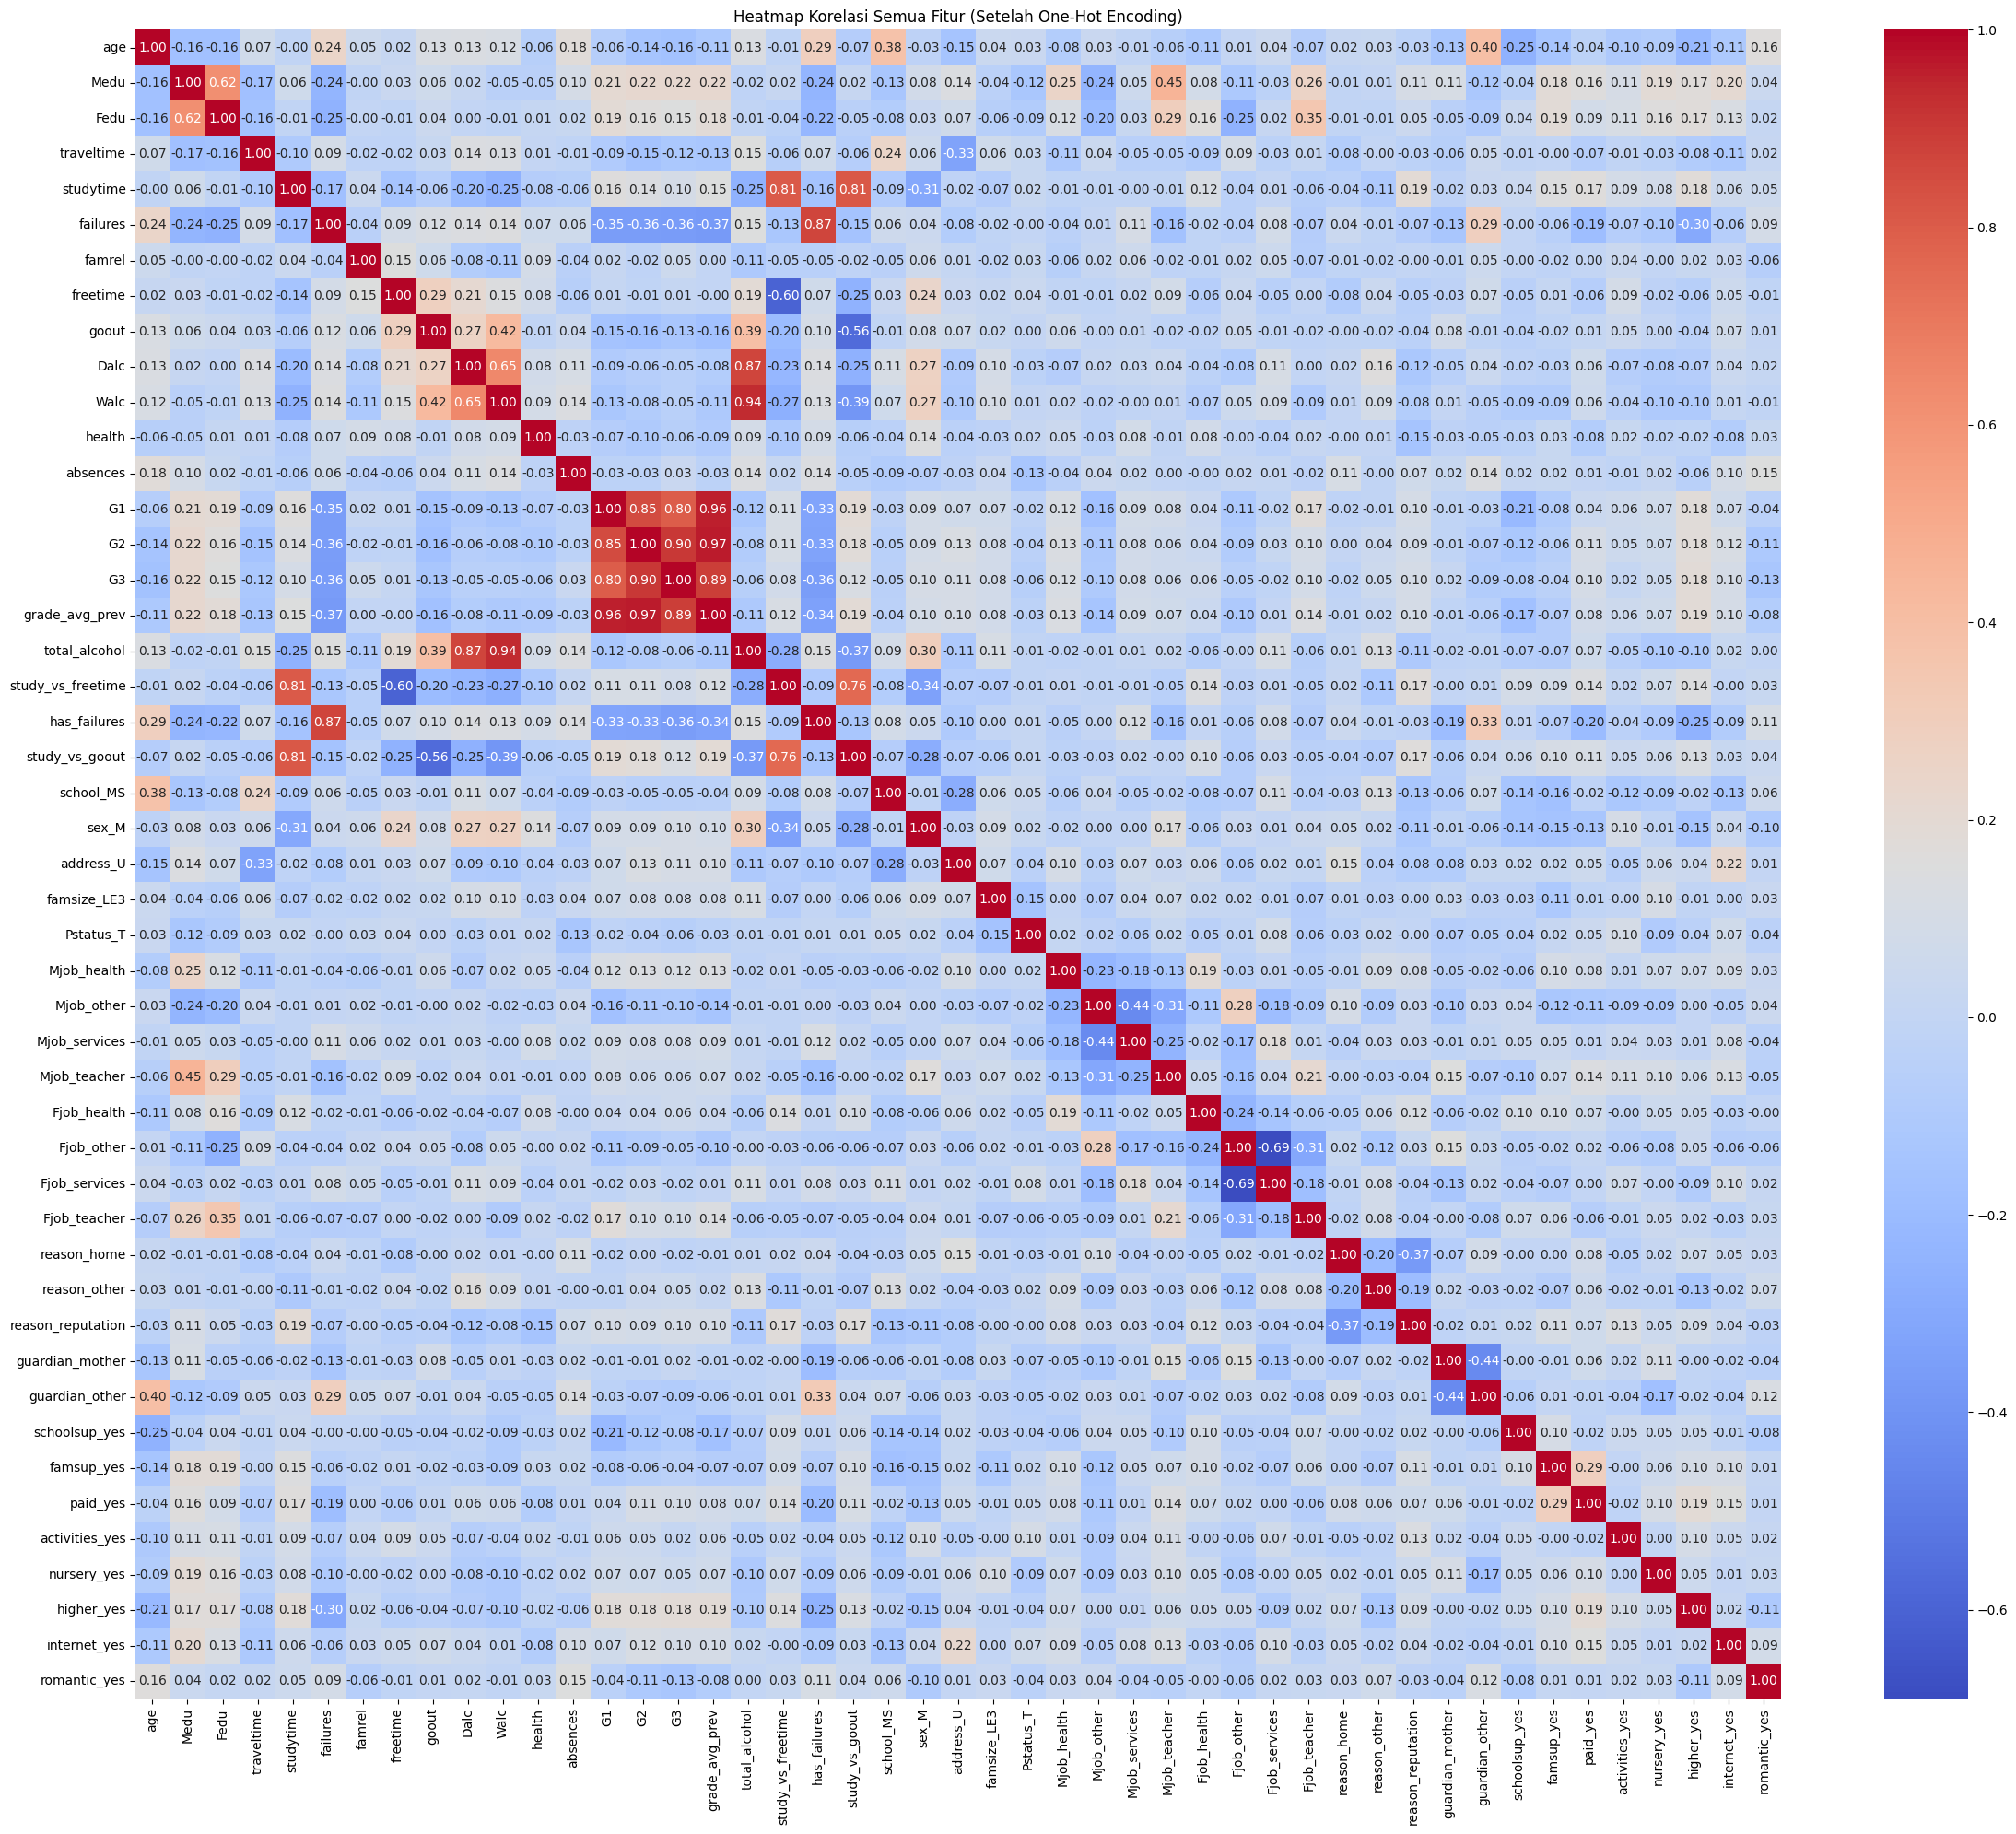
\includegraphics[width=0.8\textwidth]{images/Heatmap.png}
    \caption{Heatmap korelasi antar fitur}
\end{figure}

\subsection{Rekayasa Fitur (Feature Engineering)}
Daripada hanya menggunakan fitur asli, kami membuat fitur-fitur baru yang lebih informatif. Contohnya, \texttt{grade\_avg\_prev} (rata-rata G1 dan G2) dibuat untuk menangkap sinyal kinerja akademik sebelumnya dalam satu variabel kuat. Langkah ini relevan karena seringkali kombinasi fitur memberikan informasi yang lebih berpengaruh daripada fitur individual.
\begin{figure}[h!]
    \centering
    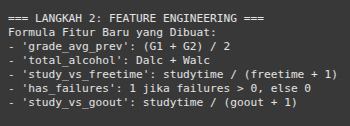
\includegraphics[width=0.8\textwidth]{images/FeatureEng.png}
    \caption{Fitur Baru yang Dibuat dari Data Asli}
\end{figure}

\subsection{One-Hot Encoding}
Model machine learning memerlukan input numerik. Fitur-fitur kategorikal seperti \texttt{sex} (`F'/`M') atau \texttt{higher} (`yes'/`no') diubah menjadi format biner (0 dan 1) melalui One-Hot Encoding. Transformasi ini wajib dilakukan agar algoritma dapat memproses semua informasi yang tersedia dalam dataset.
\begin{figure}[h!]
    \centering
    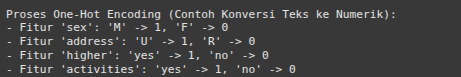
\includegraphics[width=0.8\textwidth]{images/OHE.png}
    \caption{One-Hot Encoding untuk fitur dengan value non-numerik}
\end{figure}

\vspace{0.5cm}
Setelah dataset dipahami dan diproses, fondasi telah siap untuk tahap inti proyek: pembangunan dan evaluasi model-model machine learning.
